
\documentclass[11pt,a4paper]{article}
\usepackage[utf8]{inputenc}
\usepackage[T1]{fontenc}
\usepackage{lmodern}
\usepackage{amsmath,amssymb,amsthm}
\usepackage{graphicx}
\usepackage{geometry}
\geometry{margin=1in}
\title{Optimization Methods with External Mesh (Code\_v2)}
\author{Fachseminar Report}
\date{\today}
\begin{document}
\maketitle
\section*{Overview}
This report summarizes the Ex3 reduced optimal control problem using an external mesh with a circular control region.
\section{Problem and Discretization}
We consider $\Omega=(0,1)^2$, $y$ solving $-\Delta y=\chi_{\omega}u$ with $y=0$ on $\partial\Omega$, and objective $F(u)=\tfrac{1}{2}\|y-y_d\|^2+\tfrac{\beta}{2}\|u\|^2$. Finite elements: CG1 for state/control; operators assembled from XDMF subdomain tags.
\section{Optimization Methods}
Barzilai--Borwein, fixed-step GD with $\alpha=1/L$, and Nesterov acceleration are applied in the control space with inner product induced by $M_U$.
\section{Figures}
\begin{figure}[h!]\centering
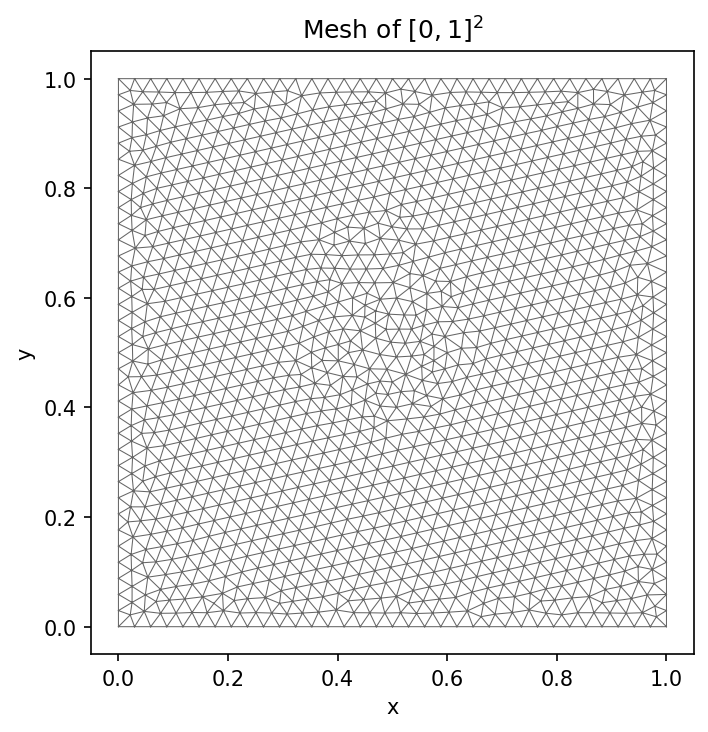
\includegraphics[width=0.45\textwidth]{mesh.png}\hfill
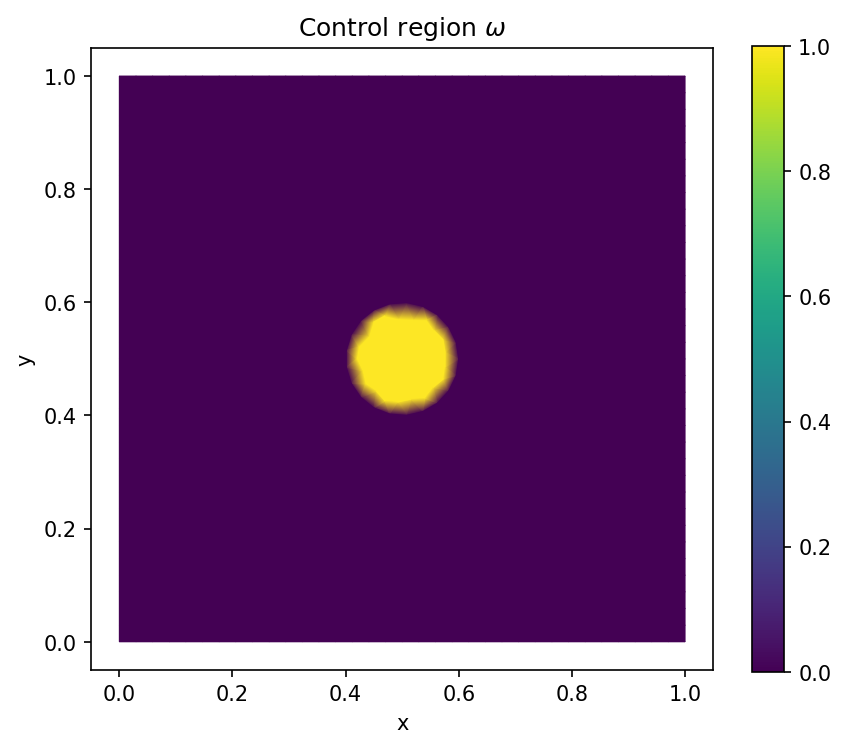
\includegraphics[width=0.45\textwidth]{omega.png}
\caption{Mesh and circular $\omega$.}\end{figure}
\begin{figure}[h!]\centering
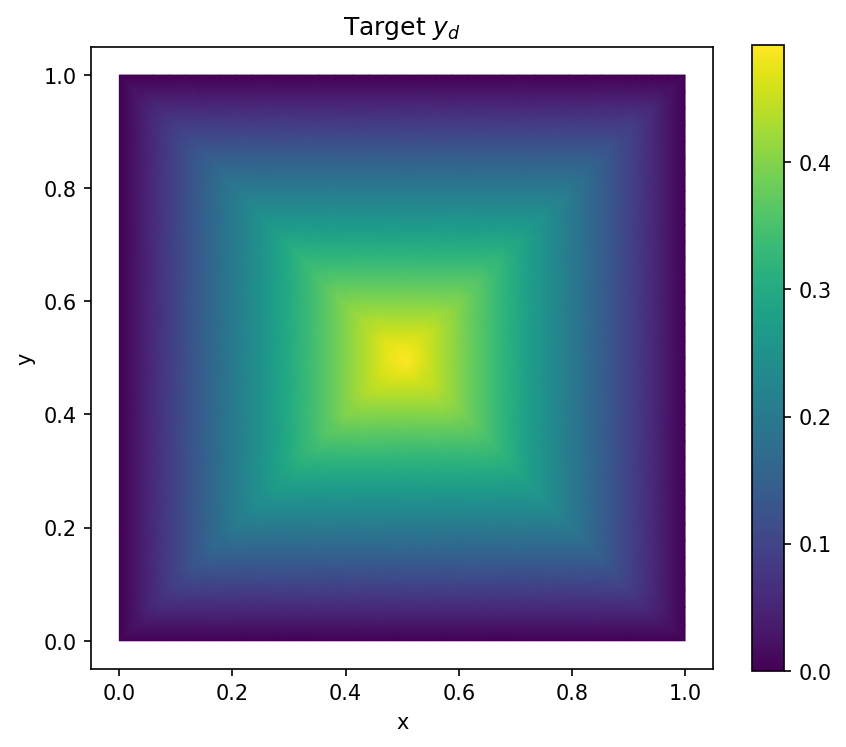
\includegraphics[width=0.45\textwidth]{y_d.png}\hfill
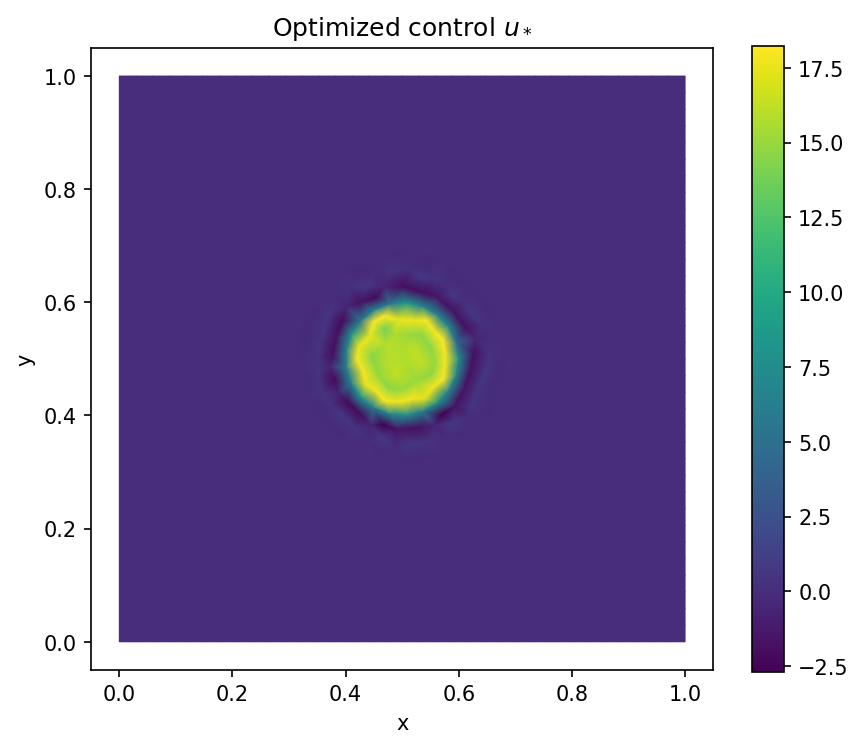
\includegraphics[width=0.45\textwidth]{u_opt.png}
\caption{Target $y_d$ and optimized control $u_*$.}\end{figure}
\begin{figure}[h!]\centering
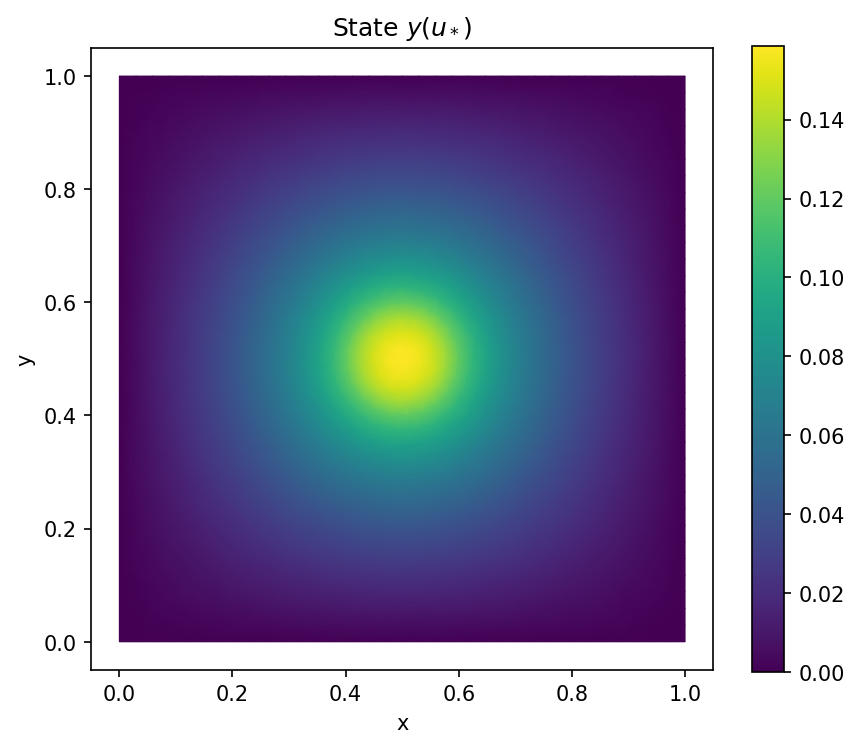
\includegraphics[width=0.45\textwidth]{y_opt.png}\hfill
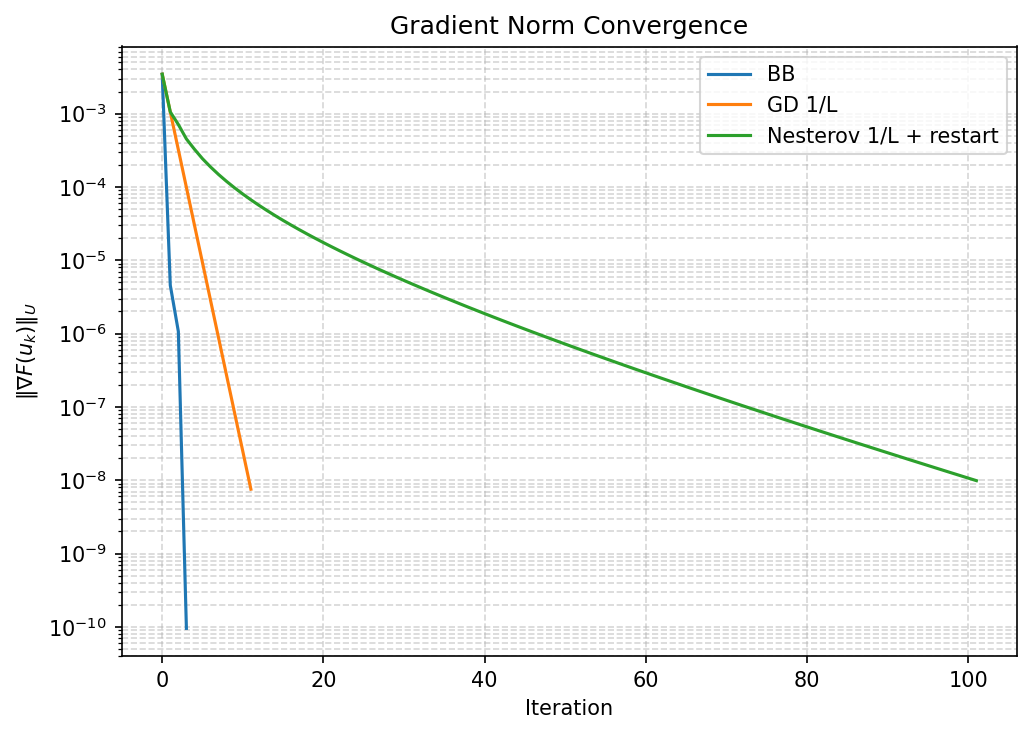
\includegraphics[width=0.45\textwidth]{grad_norm.png}
\caption{State $y(u_*)$ and gradient norm convergence.}\end{figure}
\begin{figure}[h!]\centering
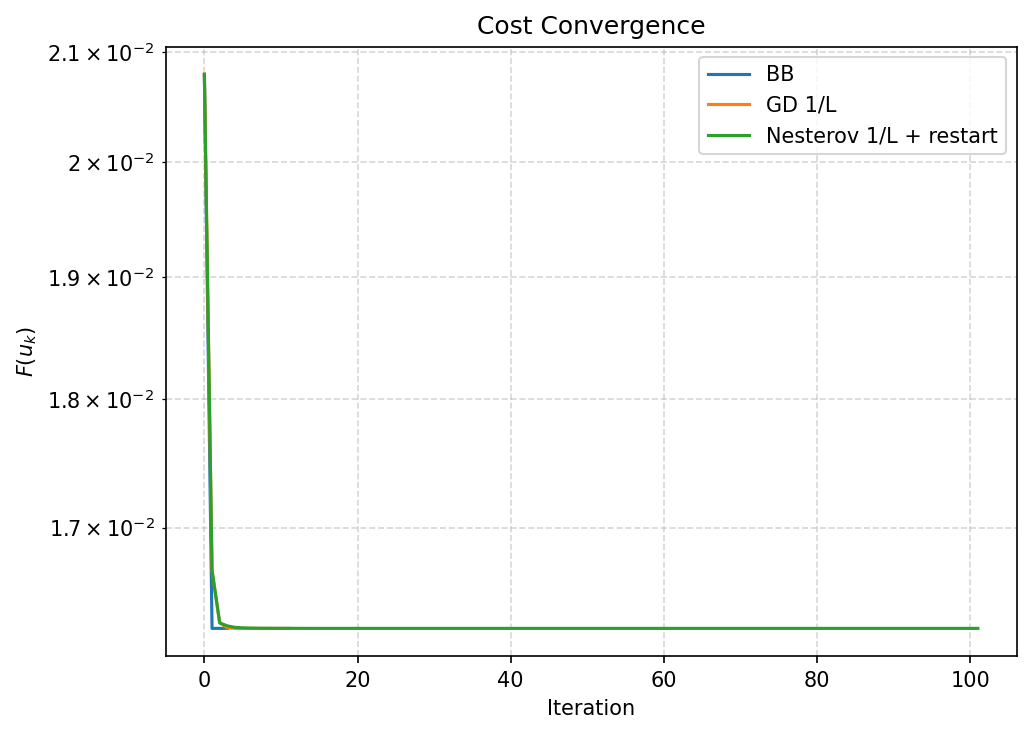
\includegraphics[width=0.45\textwidth]{cost.png}
\caption{Objective convergence.}\end{figure}
\end{document}
